\Chapter{Numerikus számítások és eredményeik}

A numerikus számításoknak megvalósításának egy elterjedt eszköze a C programozási nyelv. Az irodalomban különféle ajánlásokat találhatunk az egyes számítási módszerek elkészítésére vonatkozóan \cite{numericalrecipes}.

A fejezet bemutatja a teljesítményösszehasonlítás alapjául szolgáló három numerikus számítást, és az azokkal kapott eredményeket. Mindegyik esetében először egy rövid matematikai bevezetés található, amely leírja, hogy milyen jellegű problémáról van szó, és az hogyan oldható meg. Ezt követi a C majd a Rust nyelvű implementáció. A szakaszok végén megtekinthetjük grafikonokon a futtatások eredményét.

\Section{Valós értékek és vektorok ábrázolása}

Az algoritmusok futási idejének vizsgálata előtt érdemes megnézni, hogy a valós értékek (mint lebegőpontos számok), illetve a vektorok milyen formában szerepelnek majd a C és a Rust nyelvű implementációkban.

Lebegőpontos számok ábrázolását a Rust az IEEE-754-es szabványnak megfelelően végzi \cite{ieee}. Az egyszeres pontosságú lebegőpontos számokat az \lstinline{f32}, a dupla pontosságú lebegőpontos számokat pedig az \lstinline{f64} típusok szolgáltatják. C-ben ez nincs specifikálva, de általában az IEEE szabványát követi. Az egyszeres pontosságú a \lstinline{float}, a dupla pontosságú lebegőpontos szám a \lstinline{double} típussal reprezentálható.
%https://doc.rust-lang.org/book/ch03-02-data-types.html

A Rust nyelven implementált rendezési eljárások esetén a beépített \lstinline{Vec} adatszerkezetet használtam, melynek működéséhez hasonló saját típust definiáltam C-ben is. Ugyanakkor megemlítendő, hogy a C-s \lstinline{Vec} típus nem implementálja a Rustban meglévő vektor típus által implementált összes metódust, csak azt azokat, amelyek a dolgozatban bemutatott módszerek által használtak.
%https://doc.rust-lang.org/stable/nomicon/vec-alloc.html
\cppstyle{\begin{lstlisting}[language=c++]
typedef struct Vec {
  float *elements;
  size_t len;
  size_t capacity;
}

void vec_init(Vec *vec, size_t with_capacity) {
    vec->elements =
        (float*)malloc(with_capacity * sizeof(float) );
    vec->len = 0;
    vec->capacity = with_capacity;
}

void vec_insert(Vec *vec, float element) {
    if (vec->len == vec->capacity) {
        vec->capacity *= 2;
        vec->elements =
            (float *)realloc(vec->elements, vec->capacity * sizeof(float) );
    }
    vec->elements[vec->len++] = element;
}

Vec vec_copy(Vec *original_vec) {
    Vec new_vec;
    vec_init(&new_vec, original_vec->capacity);
    
    for (unsigned i = 0; i < original_vec->len; i++) {
        vec_insert(&new_vec, original_vec->elements[i]);
    }
    return new_vec;
}

void vec_free(Vec *vec) {
    free(vec->elements);
    vec->elements = NULL;
    vec->len = vec->capacity = 0;
}
\end{lstlisting}}

\Section{Numerikus integrálás}

A numerikus integrálás célja, hogy egy határozott integrál értékét közelítsük valamilyen pontossággal. Erre többféle módszer is adódik, amelyek közül a következő szakaszokban a trapéz szabályt és a Simpson formulát láthatjuk.

\SubSection{Trapézszabály}

\subsubsection{Rövid matematikai bevezetés}

A trapézszabály határozott integrálok meghatározására alkalmas közelítő módszer, amely egy adott intervallumba eső függvénygörbe alatti területet a függvénygörbe (vég)pontjaira illesztett trapézzal közelíti. Azaz, ha $a$ és $b$ számok az intervallum végpontjai, akkor a közelítő integrál értéke az alábbi formában becsülhető
\[
\int_{a}^{b} \! f(x) \, \textrm{d} x \approx (b - a) \cdot \frac{f(a) + f(b)}{2}.
\]

\subsubsection{C nyelvű referencia-implementáció}
A függvény \lstinline{parameter_function}-t használja egy függvényérték kiszámításához egy adott \lstinline{x} pontban.
\cppstyle{\begin{lstlisting}[language=c++]
float trapedozial_rule(float a, float b, int n) {
    float x;
    float s;
    float h;
    int i;

    h = (b - a) / n;
    x = a;
    b = 0.0;

    for (i = 0; i < n; i++) {
        x += h;
        s += parameter_function(x);
    }
    return 0.5 * (parameter_function(a) + 2.0 * s + parameter_function(b));
}
\end{lstlisting}}
A \lstinline{parameter_function} ebben az esetben az említett \(x^2 + 1\) függvény.

\subsubsection{Az algoritmus egy implementációja Rustban}

A Rust nyelvű implementáció nagyon hasonló. A lényeges különbség a mutable és immutable változók elkülönítése, illetve az \lstinline{n} változó típusának explicit castolása \lstinline{f32}-ként az osztás elvégzéséhez. A Rust nem végez automatikus típuskonverziót.
\begin{lstlisting}[language=Rust, style=boxed]
pub fn trapedozial_rule(a: f32, b: f32, n: i32) -> f32 {
    let mut x: f32;
    let mut s: f32;
    let h: f32;

    h = (b - a) / (n as f32);
    x = a;
    s = 0.0;

    for _ in 1..n {
        x += h;
        s += parameter_function(x);
    }
    return ((b - a) / n as f32) * 0.5 * (parameter_function(a)
           + 2.0 * s + parameter_function(b));
}
\end{lstlisting}

Ennél a közelítésnél külön vizsgálandó a kapott eredmény pontossága. Azért, hogy előre rögzítsük, hogy milyen pontosságot várunk el, a következőkben bemutatásra kerülő iteratív trapézszabályt célszerű alkalmazni.

\SubSection{Iteratív trapézszabály}

\subsubsection{Rövid matematikai bevezetés}

Az iteratív trapézszabály a trapézszabályra épül. Lényege, hogy a függvénygörbe alatti területre illesztett trapézok számát iteratívan növeli, így minden iterációban egyre jobb közelítést ad. A számítógép implementációk esetén ez a finomítási folyamat akkor áll meg, amikor az elmúlt iterációban nem változott jelentősen a közelítés értéke.

\subsubsection{C nyelvű referencia-implementáció}
A C nyelvű implementációban az iterációk maximális számát az \lstinline{j_max} paraméter szabályozza. Visszatér, ha az előző két iterációban kapott értékek között nincs \lstinline{EPS}-től nagyobb eltérés.
\cppstyle{\begin{lstlisting}[language=c++]
float q_trapedozial_rule(float a, float b, int j_max) {
    const float EPS = 1e-8;
    const int J_MIN_ITERATION_COUNT = 5;

    float s = 0.0;
    float olds;

    olds = -1e-29;
    for (int j = 0; j < j_max; j++) {
        s = trapedozial_rule(a, b, j);
        if (j > J_MIN_ITERATION_COUNT) {
            if (abs_float(s - olds) < EPS * abs_float(olds) ) {
                if ( (s == 0.0) && (olds == 0.0) ) {
                    return s;
                }
            }
        }
    }
    return s;
}
\end{lstlisting}}

\subsubsection{Az algoritmus egy implementációja Rustban}

Az algoritmus implementációja hasonló Rustban is, mindösszesen az olyan szintaktikai különbségek vannak, mint a zárójelezés elhagyása a \lstinline{for} és az \lstinline{if} szerkezetekben. Egyébiránt teljesen megegyező módon működik.
\begin{lstlisting}[language=Rust]
pub fn q_trapedozial_rule(a: f32, b: f32, j_max: i32) -> f32 {
    const EPS: f32 = 1e-8;
    const J_MIN_ITERATION_COUNT: i32 = 5;

    let mut s: f32 = 0.0;
    let olds: f32;

    olds = -1e-29;
    for j in 0..j_max {
        s = trapedozial_rule(a, b, j);
        if j > J_MIN_ITERATION_COUNT {
            if (s - olds).abs() < EPS * olds.abs() {
                if s == 0.0 && olds == 0.0 {
                    return s;
                }
            }
        }
    }
    return s;
}
\end{lstlisting}

\subsubsection{Futtatások eredményei}

A futtatások eredményeit \aref{fig:iterative_trapez}. ábrán láthatjuk. Jól láthatóan a módszer futási ideje négyzetes növekedést mutat a vizsgált szakaszon. Jelentős futásidőbeli eltérés a három implementáció között, amely azzal indokolható, hogy a számítások elemi műveleteket használnak csak, így közel azonos kódra fordulnak.

\begin{figure}[h!]
\centering
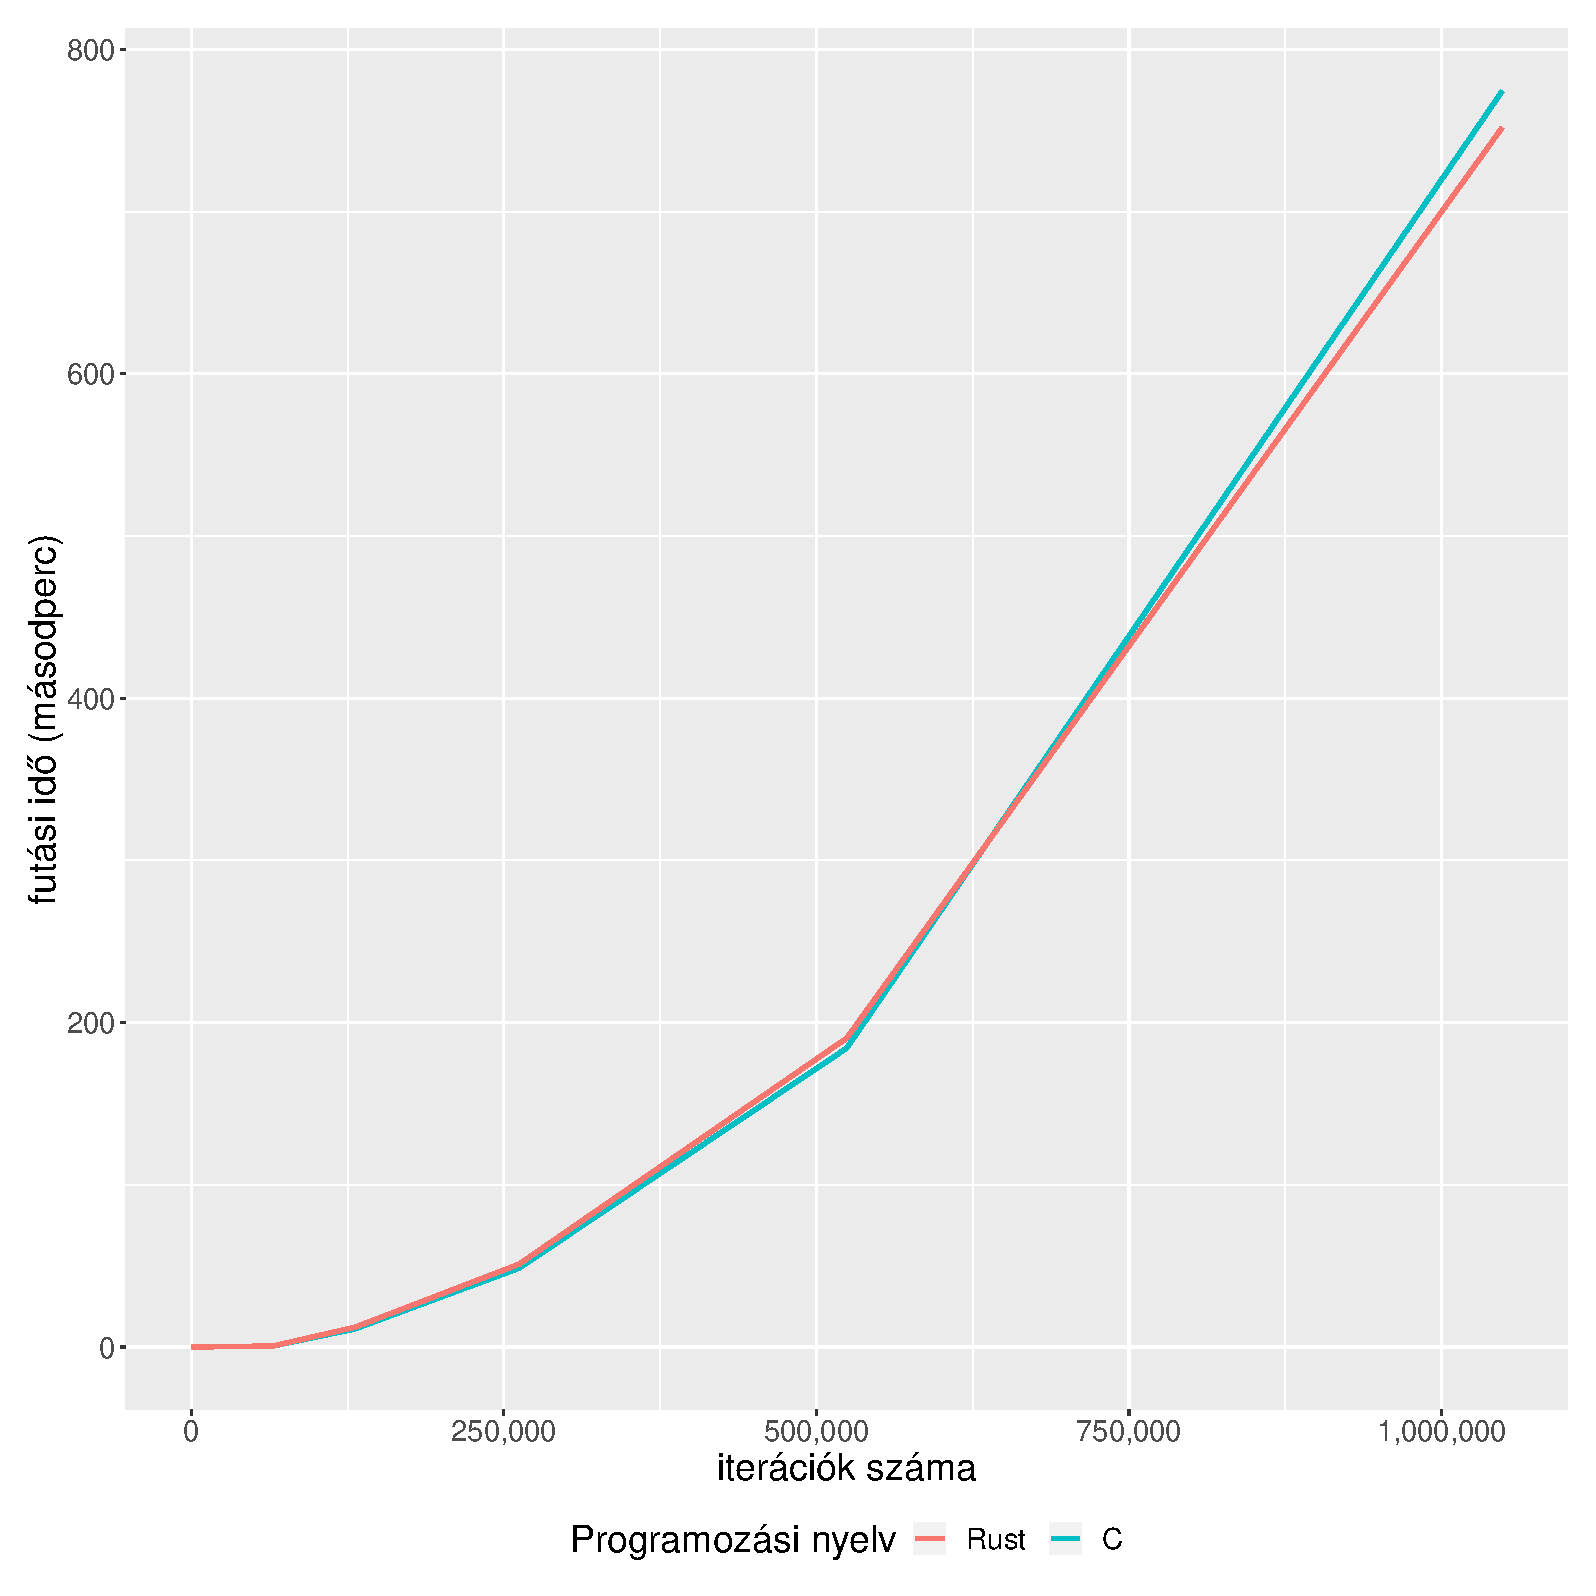
\includegraphics[width=15.5cm]{kepek/trapedozial_rule_run.eps}
\caption{Az iteratív trapézszabály futási ideje az iterációk függvényében}
\label{fig:iterative_trapez}
\end{figure}

\SubSection{Iteratív Simpson-módszer}

\subsubsection{Rövid matematikai bevezetés}

A Simpson-módszer a trapézszabályon alapul úgy, hogy a részintervallumok végpontjaihoz súlyokat rendel. A Simpson-módszert használja, vagyis az iteratív trapézszabályhoz hasonlóan finomítja egyre jobban a közelítést minden iterációban \cite{simpson}.

\subsubsection{C nyelvű referencia-implementáció}

A Simpson-módszer implementációja hasonló az iteratív trapézszabályékhoz, a különbséget a közelítő érték kiszámításához használatos formula jelenti.
\cppstyle{\begin{lstlisting}[language=c++]
float q_simpsons_rule(float a, float b, int j_max) {
    const float EPS = 1e-9;
    const int J_MIN_ITERATION_COUNT = 5;

    float s = 0.0;
    float st;
    float ost;
    float os;

    os = -1e-29;
    ost = os;

    for (int j = 0; j < j_max; j++) {
        st = trapedozial_rule(a, b, j);
        s = (4.0 * st - ost) / 3.0;
        if (j > J_MIN_ITERATION_COUNT) {
            if (abs_float(s - os) < EPS * abs_float(os)
                || (s == 0.0 && os == 0.0) ) {
                return s;
            }
        }
        os = s;
        ost = st;
    }
    return s;
}
\end{lstlisting}}

\subsubsection{Az algoritmus egy implementációja Rustban}

Az algoritmus Rust nyelvű implementációja, jelentős különbségek ebben az esetben sincsenek.
\begin{lstlisting}[language=Rust]
pub fn q_simpsons_rule(a: f32, b: f32, j_max: i32) -> f32 {
    const EPS: f32 = 1e-9;
    const J_MIN_ITERATION_COUNT: i32 = 5;

    let mut s: f32 = 0.0;
    let mut st: f32;
    let mut ost: f32;
    let mut os: f32;

    os = -1e-29;
    ost = os;

    for j in 0..j_max {
        st = trapedozial_rule(a, b, j);
        s = (4.0 * st - ost) / 3.0;
        if j > J_MIN_ITERATION_COUNT {
            if (s - os).abs() < EPS * os.abs() || (s == 0.0 && os == 0.0) {
                return s;
            }
        }
        os = s;
        ost = st;
    }
    return s;
}
\end{lstlisting}

\subsubsection{Futtatások eredményei}

A kapott futási időket \aref{fig:iterative_simpson}. ábrán láthatjuk. Ez alapján itt is megállapítható, hogy ilyen jellegű számítások esetében a Rust nyelvű megvalósítás a C nyelvűvel közel azonos futási időket eredményez.

\begin{figure}[h!]
\centering
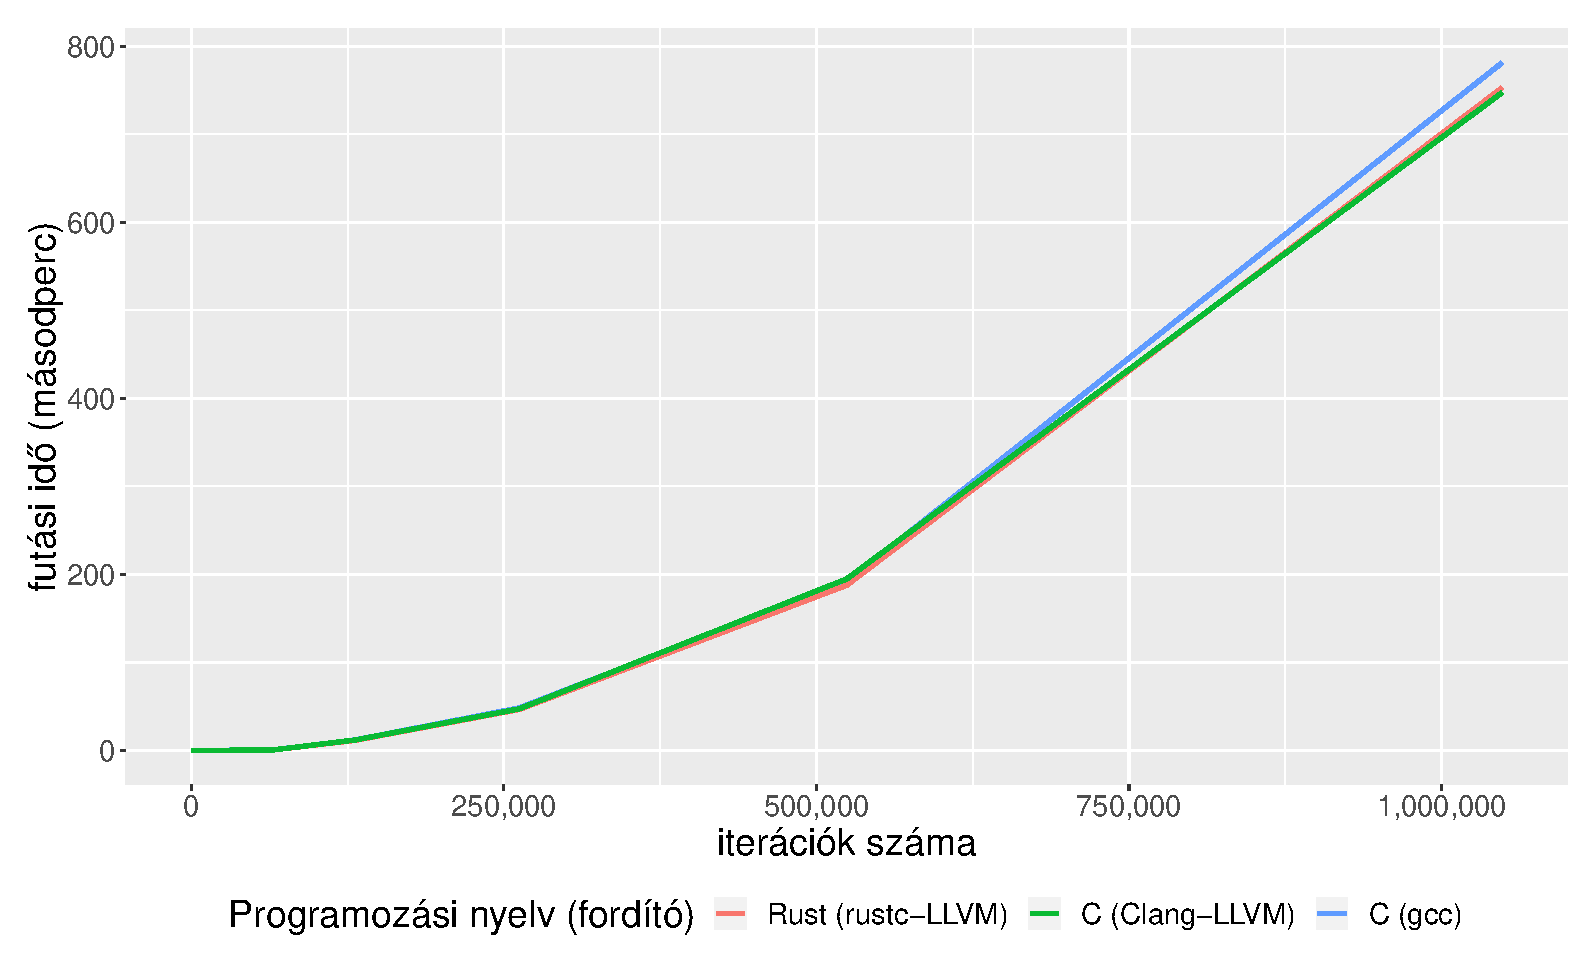
\includegraphics[width=15.5cm]{kepek/simpsons_rule_run.eps}
\caption{Az iterative Simpson formula alkalmazásával kapott futási idők}
\label{fig:iterative_simpson}
\end{figure}

\Section{Rendezés}

Rendezőalgoritmusok alkalmazására gyakran szükség van, mivel rendezett adatszerkezetekben a keresési műveletek hatékonyabban elvégezhetők. A rendezésre számos lehetőség adódik, amelyekből a következőkben a kupacrendezés, shell rendezés és a gyorsrendezés esetét fogjuk megvizsgálni.

\SubSection{Kupacrendezés}

A kupacrendezés a nevét a benne használt kupac (\textit{heap}) adatszerkezetről kapta \cite{heapsort}.

\subsubsection{Rövid matematikai bevezetés}

A kupacrendezés két részre osztja az inputot: egy rendezett és egy nem rendezett részre. A gyökérelem (legnagyobb elem) megkeresésével és a rendezett részbe mozgatásával egyre csökkenti a nem rendezett rész méretét. Legrosszabb esetben is \[ T(n) = \Theta(n \log n)\] időkomplexitással rendelkezik, ahol az $n$ a rendezendő elemek számát jelöli.

\subsubsection{C nyelvű referencia-implementáció}

\cppstyle{\begin{lstlisting}[language=c++]
void heapify(Vec *a, unsigned n, unsigned i) {
    unsigned largest = i;
    unsigned l = 2 * i + 1;
    unsigned r = 2 * i + 2;

    if ((r < n) && (a->elements[i] < a->elements[l])) {
        largest = l;
    }

    if ((r < n) && (a->elements[largest] < a->elements[r]) ) {
        largest = r;
    }

    if (largest != i) {
        SWAP(float, a->elements[largest], a->elements[i]);
        heapify(a, n, largest);
    }
}

void heapsort(unsigned n, Vec *a) {
    unsigned i = n;
    while (i > 0) {
        heapify(a, n, i);
        i -= 1;
    }

    i = n - 1;
    while (i > 0) {
        SWAP(float, a->elements[0], a->elements[i]);
        heapify(a, i ,0);
        i -= 1;
    }
}
\end{lstlisting}}
A rendezendő elemek egy \lstinline{Vec} struktúrába kerülnek. Erre azért van ilyen formában szükség, hogy a kupac elemei külön mezővel hivatkozhatóak legyenek. A \lstinline{SWAP} az adott elemeket cseréli fel.

\subsubsection{Az algoritmus egy implementációja Rustban}

Kiemelendő részlet, hogy a Rust nyelvű implementációban a \lstinline{Vec} típus \lstinline{swap} metódusa került felhasználásra a vektor két elemének megcseréléséhez.
\begin{lstlisting}[language=Rust]
fn heapify(a: &mut Vec<f32>, n: usize, i: usize) {
    let mut largest: usize = i;
    let l = 2 * i + 1;
    let r = 2 * i + 2;

    if r < n && a[i] < a[l] {
        largest = l;
    }

    if r < n && a[largest] < a[r] {
        largest = r;
    }

    if largest != i {
        a.swap(largest, i);

        heapify(a, n, largest);
    }
}

pub fn heapsort(n: usize, a: &mut Vec<f32>) {
    let mut i: usize = n;
    while i > 0 {
        heapify(a, n, i);
        i -= 1;
    }

    i = n - 1;
    while i > 0 {
        a.swap(0, i);
        heapify(a, i, 0);
        i -= 1;
    }
}
\end{lstlisting}

\subsubsection{Futtatások eredményei}

Kupac-rendezés futási ideje \aref{fig:heapsort}. ábrán látható.

\begin{figure}[h!]
\centering
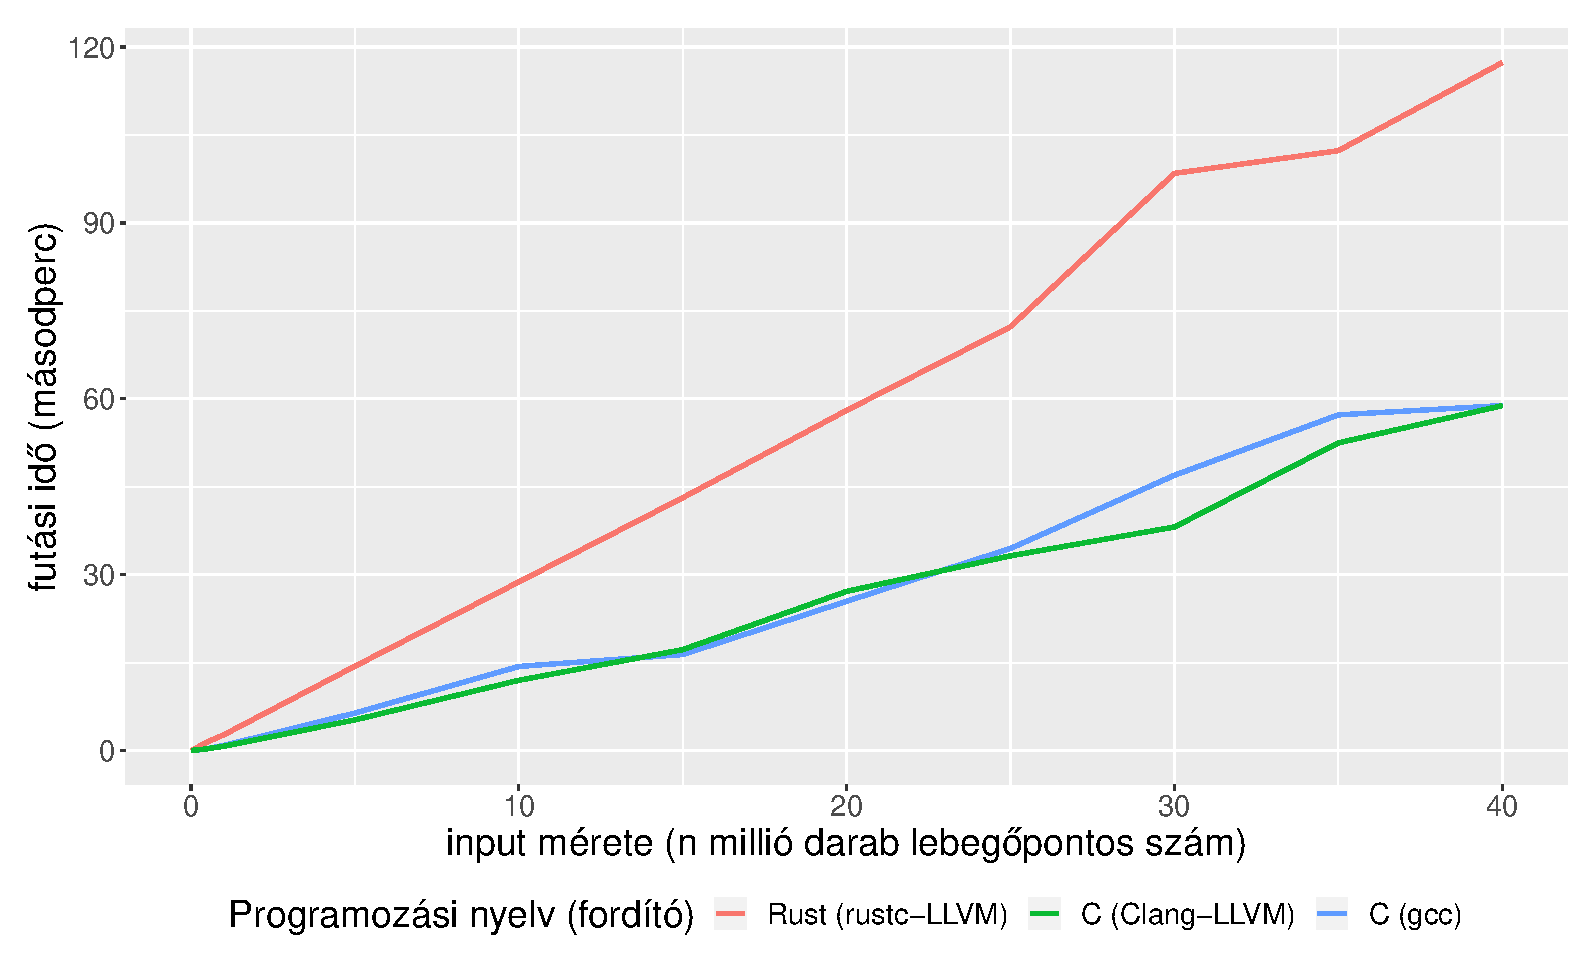
\includegraphics[width=15.5cm]{kepek/heap_sort_run.eps}
\caption{A kupacrendezés futási idejének összehasonlítása}
\label{fig:heapsort}
\end{figure}

Látható, hogy a kupac-rendezés módszerét tekintve a Rust nyelvű implementáció lassabb, mint a C-s megfelelője.

A kupac-rendezés maximális memóriafoglalását \aref{fig:heapsort_mem}. ábrán láthatjuk. A Rust és C nyelven elkészített implementációk között e tekintben az eltérések abból adódnak, hogy a Rust helyben, vektoros formában kezeli az elemeket. Így tehát a memóriaigény kisebb tud maradni, viszont emiatt a futási idő nőni fog.

\begin{figure}[h!]
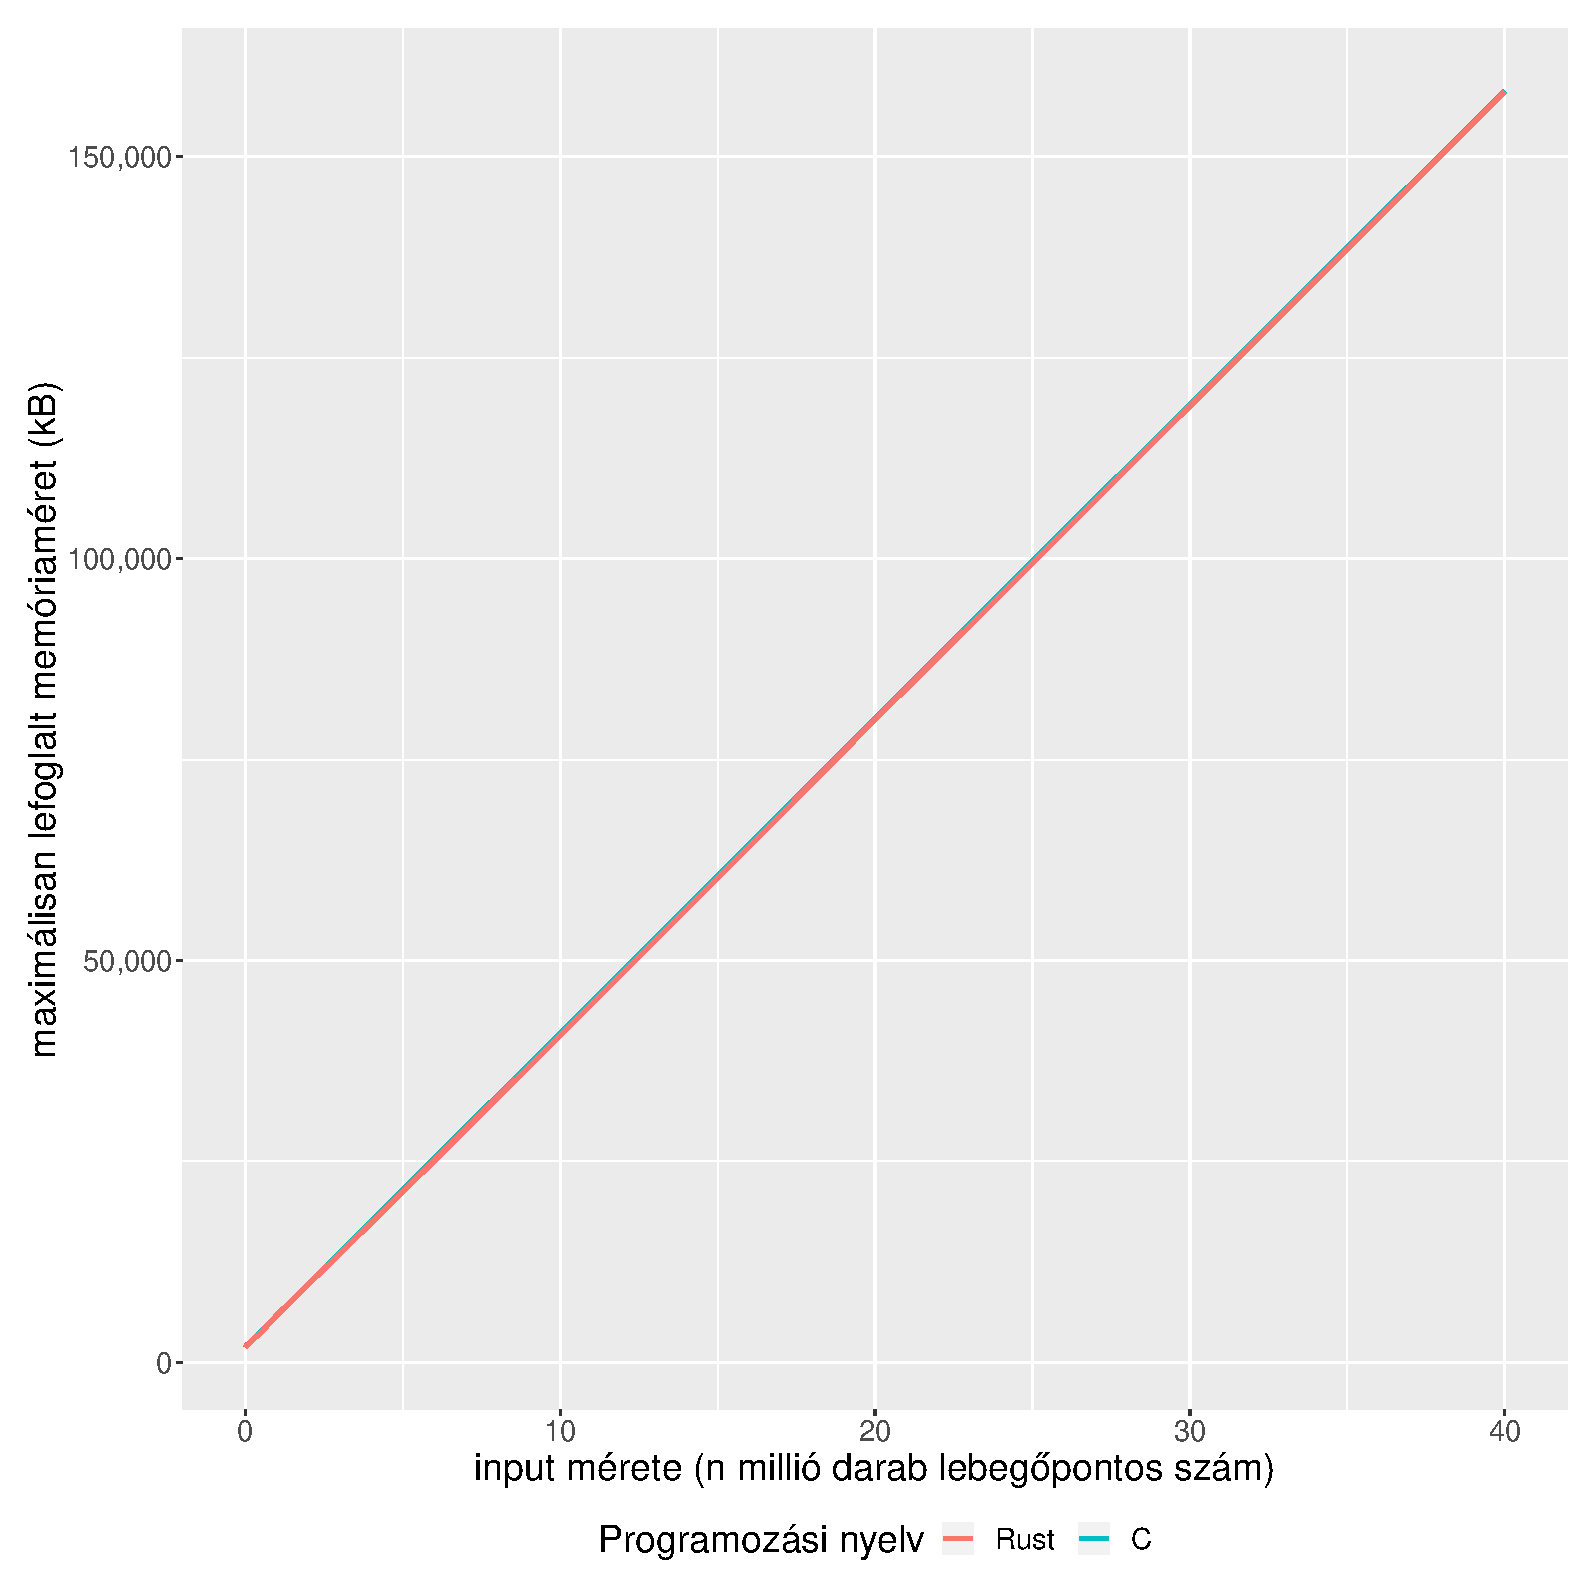
\includegraphics[width=15.5cm]{kepek/heap_sort_memory.eps}
\caption{A kupac-rendezés memóriaigénye}
\label{fig:heapsort_mem}
\end{figure}

\SubSection{Shell-rendezés}

A Shell-rendezés a buborékrendezés egy javított változatának tekinthető, amelyben az egyes iterációkban különböző távolságra lévő elemeket tudunk mozgatni \cite{shellsort}.

\subsubsection{Rövid matematikai bevezetés}

Az egymástól távoli elemek összehasonlításával kezdi a rendezést, majd a szomszédos elemek felé, egyre közelebbi elemeket összehasonlítva, és szükség szerint felcserélve azokat. Az elméleti futásidő a legjobb és az átlagos esetben:
\[ T(n) = \Theta(n \log n) \]
míg a legrosszabb esetben
\[ T(n) = \Theta(n^2)\]
időre adódik.

\subsubsection{C nyelvű referencia-implementáció}

\cppstyle{\begin{lstlisting}[language=c++]
void shell_sort(unsigned n, Vec *a) {
    int gap = (n / 2);
    float temp;
    unsigned int i;
    int j;

    while (gap > 0) {
        for (i = gap; i < n; i++) {
            temp = a->elements[i];
            
            j = i;
            while ((j >= gap) && (a->elements[(j-gap)] > temp) ) {
                a->elements[j] = a->elements[(j-gap)];
                j -= gap;
            }
            a->elements[j] = temp;
        }
        gap /= 2;
    }
}
\end{lstlisting}}
\subsubsection{Az algoritmus egy implementációja Rustban}
\begin{lstlisting}[language=Rust]
pub fn shell_sort(n: i32, a: &mut Vec<f32>) {
    let mut gap: i32 = (n / 2) as i32;
    let mut temp: f32;
    let mut j: i32;

    while gap > 0 {
        for i in gap..n {
            temp = a[i as usize];

            j = i;
            while j >= gap && a[(j - gap) as usize] > temp {
                a[j as usize] = a[(j - gap) as usize];
                j -= gap;
            }
            a[j as usize] = temp;
        }
        gap /= 2;
    }
}
\end{lstlisting}

\subsubsection{Futtatások eredményei}

Shell-rendezés futási ideje \aref{fig:shellsort}. ábrán látható.

\begin{figure}[h!]
\centering
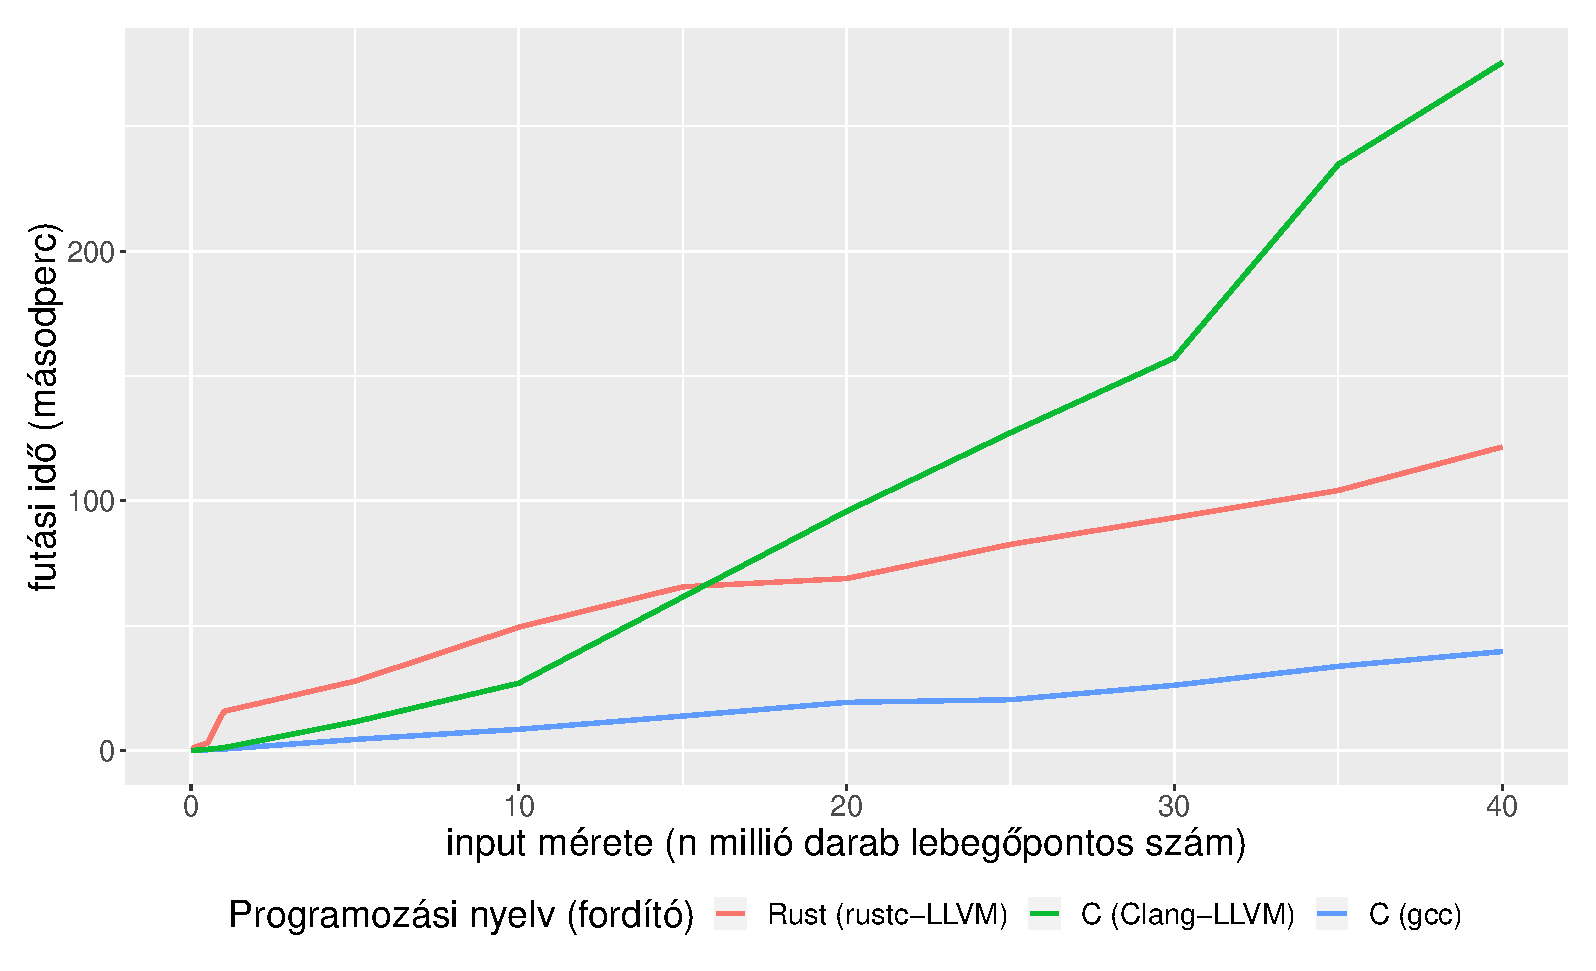
\includegraphics[width=15.5cm]{kepek/shells_sort_run.eps}
\caption{A Shell-rendezés futási ideje}
\label{fig:shellsort}
\end{figure}

Ez már egy változatosabb eredményt ad. A Rust ugyan lassabb, mint a \texttt{gcc}-vel fordított C változat, viszont 15 millió elemtől már hatékonyabbnak bizonyult, mint az LLVM-el fordított.

A maximális memóriafoglalást \aref{fig:shellsort_mem}. ábrán láthatjuk. Ez a kupacrendezéssel azonos eredményt ad, mivel a háttérben lévő adatszerkezetek is azonosak.

\begin{figure}[h!]
\centering
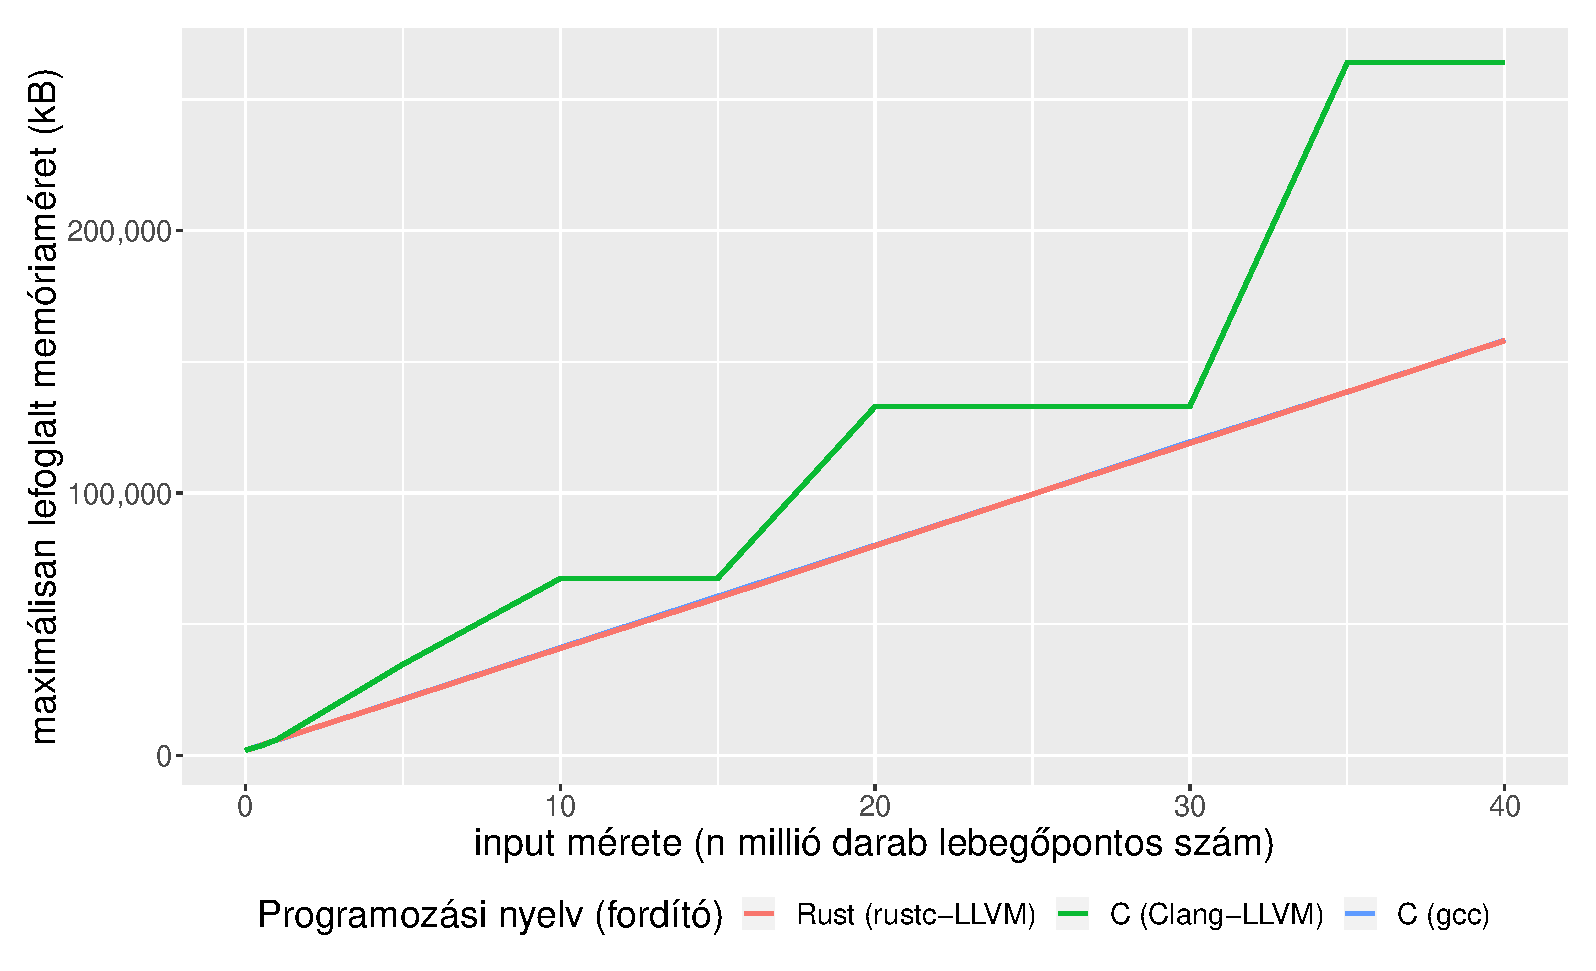
\includegraphics[width=15.5cm]{kepek/shells_sort_memory.eps}
\caption{A Shell-rendezés memóriaigénye}
\label{fig:shellsort_mem}
\end{figure}

\SubSection{Gyorsrendezés}

A gyorsrendezés (\textit{Quicksort}) az egyik leginkább elterjedt rendező algoritmus a hatékonysága és az egyszerű megvalósíthatósága miatt.

\subsubsection{Rövid matematikai bevezetés}

A gyorsrendezés egy rekurzív algoritmus, amely az „oszd meg és uralkodj” elve alapján működik. Az input elemeket két részre osztja az alapján, hogy egy kiválasztott (pivot) elemtől kisebbek, vagy nagyobbak. Az így létrejött két részre meghívásra kerül a gyorsrendezés, egészen addig, amíg egy elemű részek nem jönnek létre. Egyetlen elem mindig rendezett. Az implementációban a Robert Sedgewick ajánlásának megfelelően kerül kiválasztásra a pivot elem, így elkerülhető a legrosszabb eset, a már rendezett elemek listája \cite{sedgewickquicksort}.

Az elméleti futásidő legjobb és átlagos esetben
\[ T(n) = \Theta(n \log n), \]
a legrosszabb esetben pedig
\[ T(n) = \Theta(n^2).\]
 
\subsubsection{C nyelvű referencia-implementáció}

\cppstyle{\begin{lstlisting}[language=c++]
int partition(int low, int high, Vec *arr) {
    float pivot;

    int mid = (low + high) / 2;
    if (arr->elements[mid] < arr->elements[low]) {
        SWAP(float, arr->elements[low], arr->elements[high]);
    }

    if (arr->elements[high] < arr->elements[low]) {
        SWAP(float, arr->elements[low], arr->elements[high]);
    }

    if (arr->elements[mid] < arr->elements[high]) {
        SWAP(float, arr->elements[mid], arr->elements[high]);
    }

    pivot = arr->elements[high];

    int i;
    int j;

    i = low - 1;
	  j = high + 1;

    while (1) {
        while (1) {
            i += 1;
            if (arr->elements[i] >= pivot) {
                break;
            }
        }

        while (1) {
            j -= 1;
            if (arr->elements[j] <= pivot) {
                break;
            }
        }

        if (i >= j) {
            return j;
        }

        SWAP(float, arr->elements[i], arr->elements[j]);
    }
}

void quicksort(int low, int high, Vec *arr) {
    if (low < high) {
        int p = partition(low, high, arr);
        quicksort(low, p, arr);
        quicksort(p + 1, high, arr);
    } else {
        return;
    }
}
\end{lstlisting}}
\subsubsection{Az algoritmus egy implementációja Rustban}

\begin{lstlisting}[language=Rust]
pub fn quicksort(low: i32, high: i32, arr: &mut Vec<f32>) {
    if low < high {
        let p: i32 = partition(low, high, arr);
        quicksort(low, p, arr);
        quicksort(p + 1, high, arr);
    } else {
        return;
    }
}

fn partition(low: i32, high: i32, arr: &mut Vec<f32>) -> i32 {
    let pivot: f32;

    let mid: i32 = (low + high) / 2;
    if arr[mid as usize] < arr[low as usize] {
        arr.swap(low as usize, high as usize);
    }
    if arr[high as usize] < arr[low as usize] {
        arr.swap(low as usize, high as usize);
    }
    if arr[mid as usize] < arr[high as usize] {
        arr.swap(mid as usize, high as usize);
    }
    pivot = arr[high as usize];

    let mut i: i32;
    let mut j: i32;

    i = low - 1;
    j = high + 1;

    loop {
        loop {
            i += 1;
            if arr[i as usize] >= pivot {
                break;
            }
        }

        loop {
            j -= 1;
            if arr[j as usize] <= pivot {
                break;
            }
        }

        if i >= j {
            return j as i32;
        }

        arr.swap(i as usize, j as usize);
    }
}

\end{lstlisting}

\subsubsection{Futtatások eredményei}

Gyorsrendezés futási ideje \aref{fig:quicksort}. ábrán látható.

\begin{figure}[h!]
\centering
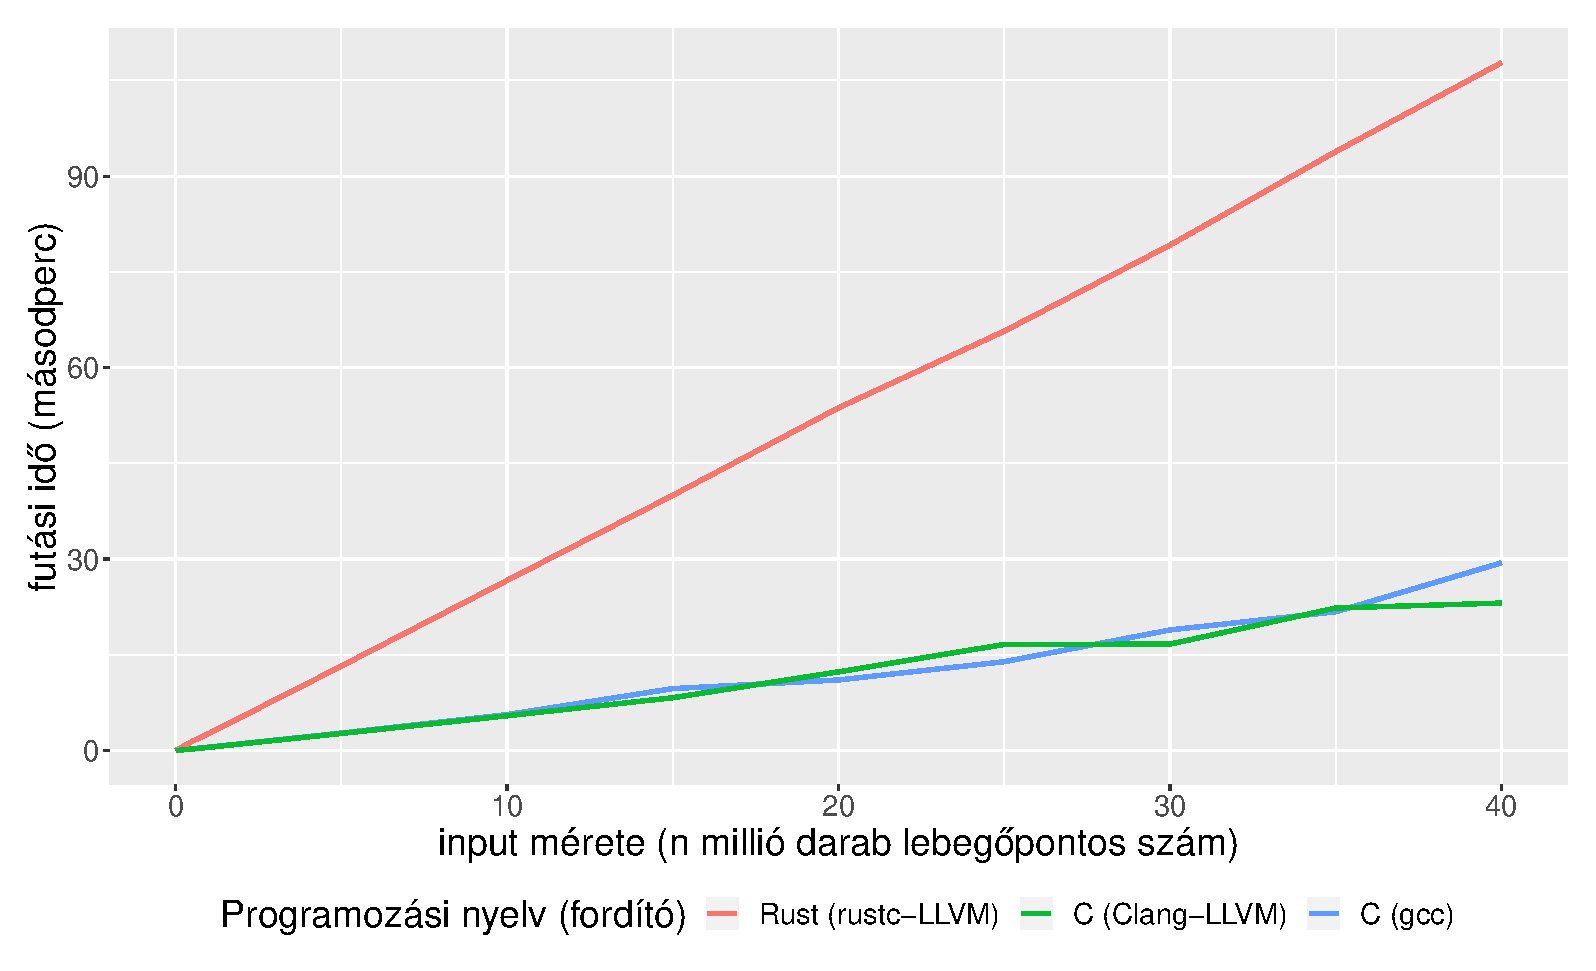
\includegraphics[width=15.5cm]{kepek/quicksort_run.eps}
\caption{A gyorsrendezés futási ideje a három vizsgált implementációban}
\label{fig:quicksort}
\end{figure}

Látható, hogy a gyorsrendezés módszerét tekintve a Rust nyelvű implementáció lassabb, mint a C-s megfelelője. A növekedés az elemszám függvényében az adott szakaszon látszólag lineáris, de határértékben az $n \cdot \log n$ függvényhez tart.

A maximális memóriafoglalás tekintetében a gyorsrendezés esetében sincs különbség az előzőekben bemutatott rendezőalgoritmusokhoz képest.

\Section{Interpoláció}

Az interpoláció célja, hogy a segítségével diszkrét pontok között tetszőleges sok folytonos érték számítható legyen.

\SubSection{Lineáris interpoláció}

Az interpolációs számítások közül a következőkben a lineáris eset vizsgálatára kerül majd sor egyváltozós esetben.

\subsubsection{Rövid matematikai bevezetés}

A lineáris interpoláció két ismert pont közötti értékeket egyenes arányossággal közelíti. Legyenek az ismert pontok az $(x_0, y_0)$ és $(x_1, y_1)$ pontok. Ekkor egy tetszőleges $x$ értékhez az $y$ érték az alábbi formában számolható
\[ y = \frac{x - x_0}{x_1 - x_0} \cdot (y_1 - y_0) + y_0, \]
ahol feltételezzük, hogy $x_0 \neq x_1$. Ha az egyenlőség teljesülne, akkor definiálhatjuk úgy a függvényt, hogy az $y_0$ értékkel térjen vissza.

\subsubsection{C nyelvű referencia-implementáció}

A lineáris interpoláció implementációja egyszerű. Ha a paraméterként kapott két pont \lstinline{x} értékei megegyeznek, akkor az első pont \lstinline{y} értékével tér vissza.
\cppstyle{\begin{lstlisting}[language=c++]
float linear_interpolation(float x1, float y1, float x0, float y0, float x) {
    float delta;
    delta = x1 - x0;
    float y;

    if (delta == 0.0) {
        y = y0;
    } else {
        y = y0 + ( (x - x0) / delta) * y1;
    }

    return y;
}
\end{lstlisting}}
\subsubsection{Az algoritmus egy implementációja Rustban}
A Rust nyelvű implementáció nem mutat az esetleges szintaktikai különbözőségeken felül más eltérést a C nyelvűtől.
\begin{lstlisting}[language=Rust]
fn linear_interpolation(x1: f32, y1: f32, x0: f32, y0: f32, x: f32) -> f32 {
    let delta: f32;
    delta = x1 - x0;
    let y;

    if delta == 0.0 {
        y = y0;
    } else {
        y = y0 + ((x - x0) / delta) * y1;
    }

    return y;
}
\end{lstlisting}

\subsubsection{Futtatások eredményei}

Lineáris interpoláció futási ideje \aref{fig:interpolation}. ábrán látható.

\begin{figure}[h!]
\centering
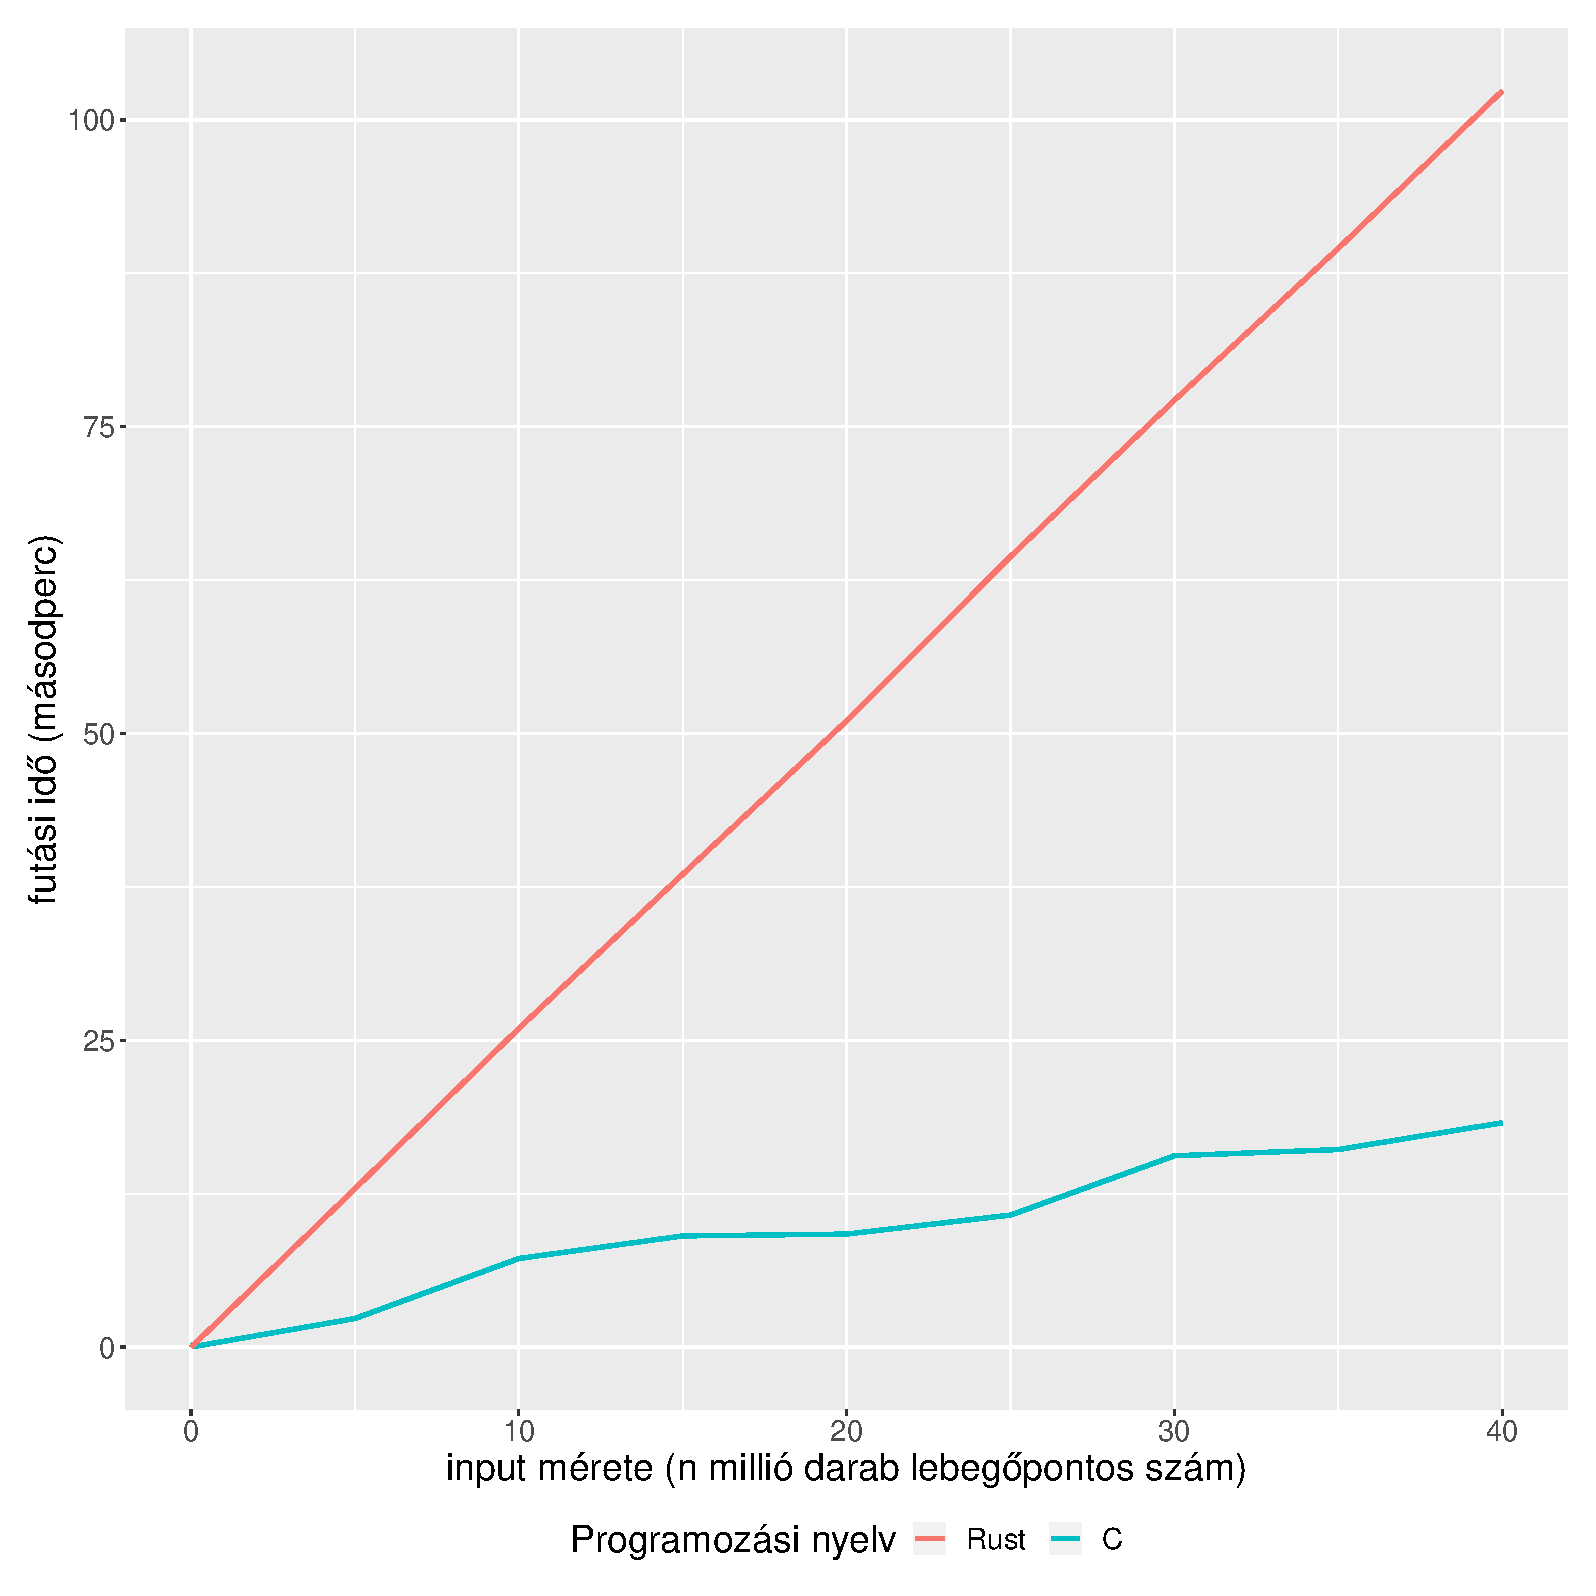
\includegraphics[width=15.5cm]{kepek/linear_interpolation_run.eps}
\caption{A lineáris interpoláció futási ideje}
\label{fig:interpolation}
\end{figure}

Látható, hogy a lineáris interpoláció módszerét tekintve a Rust nyelvű implementáció lassabb, mint a C-s megfelelője.

A lineáris interpoláció maximális memóriafoglalása \aref{fig:interpolation_mem} ábrán látható.

\begin{figure}[h!]
\centering
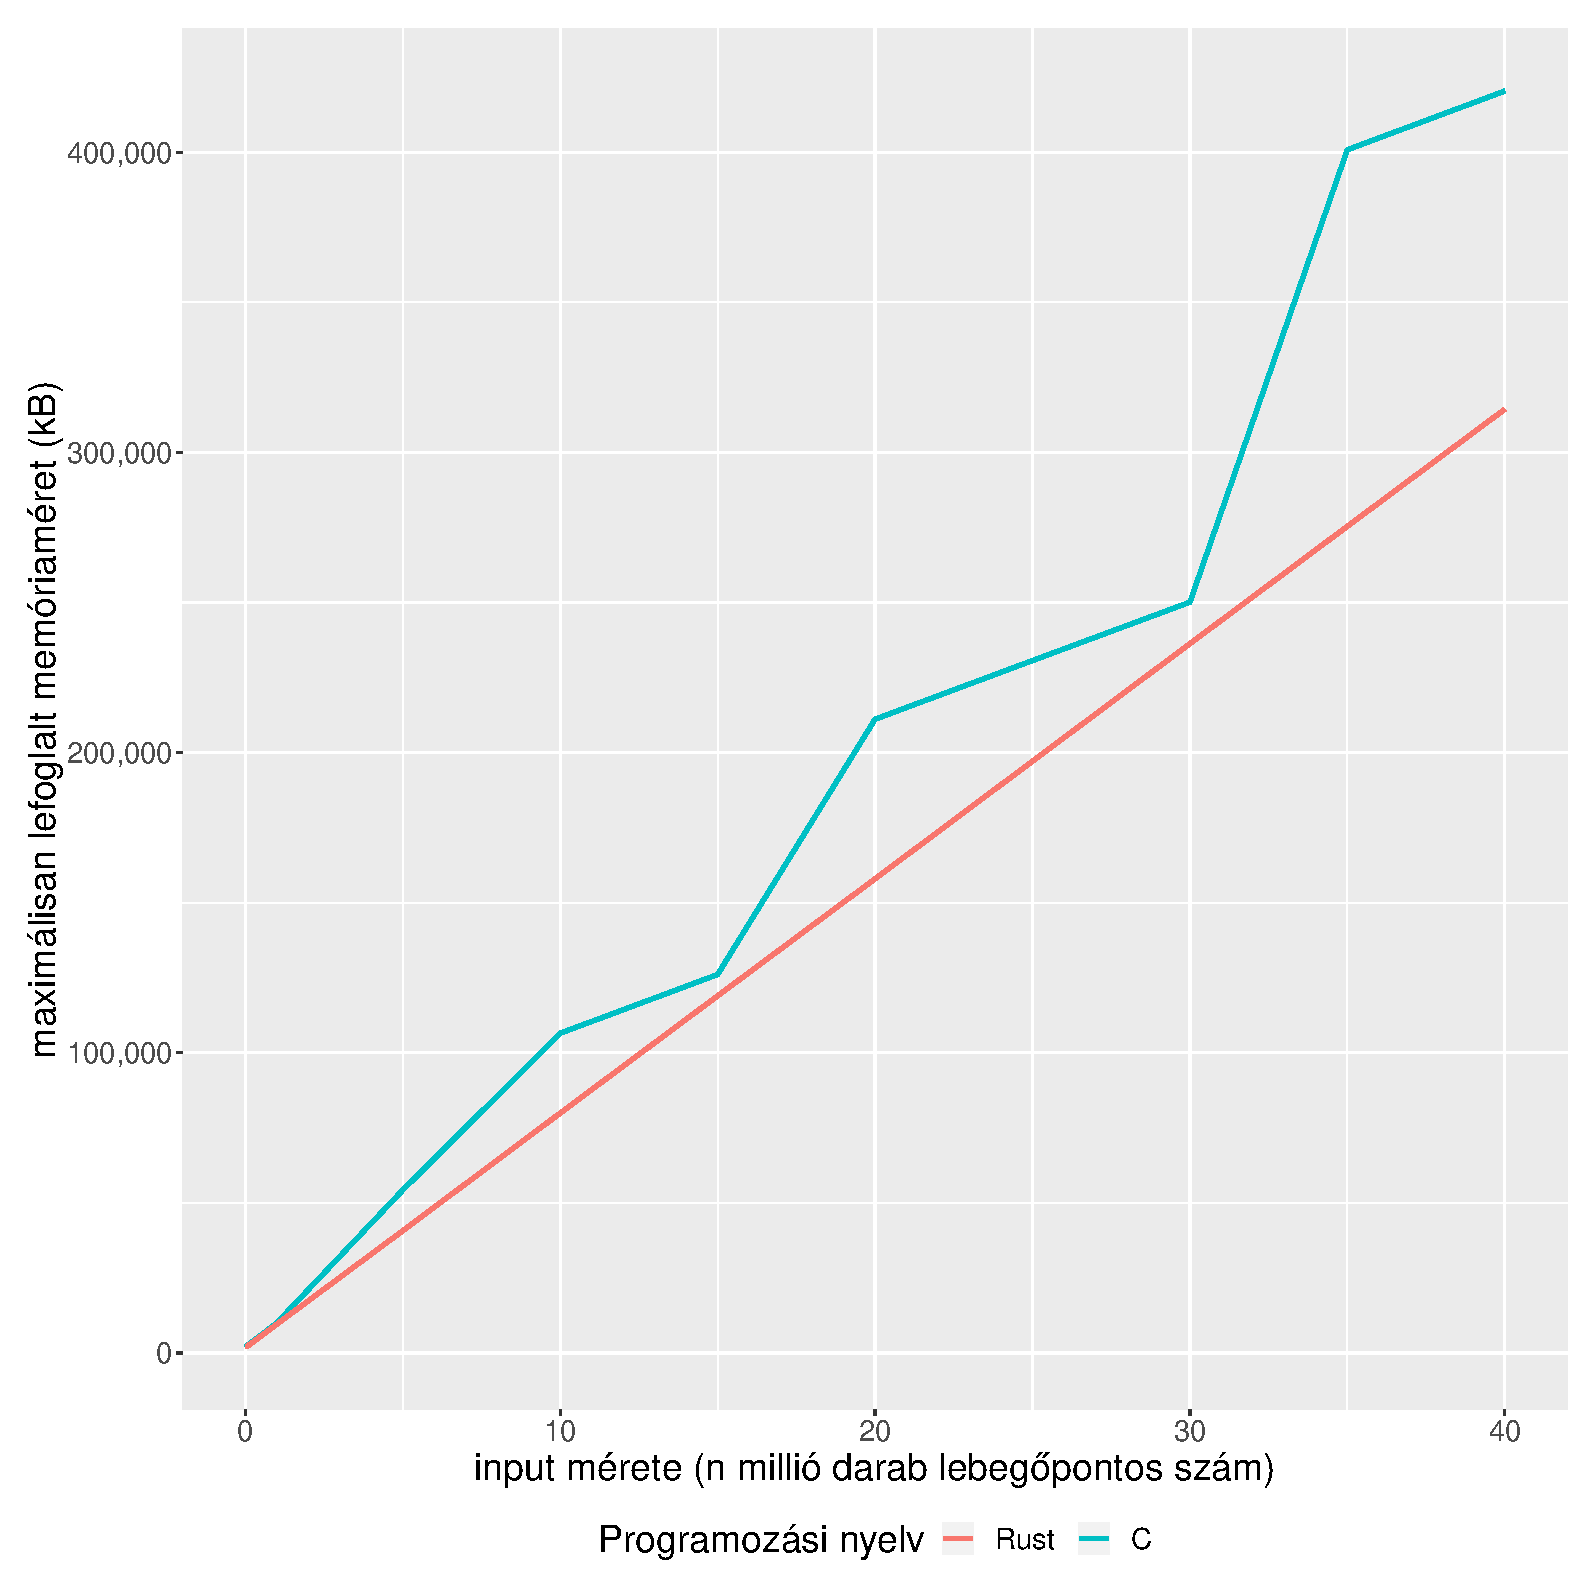
\includegraphics[width=15.5cm]{kepek/linear_interpolation_memory.eps}
\caption{A lineáris interpoláció maximális memóriaigénye}
\label{fig:interpolation_mem}
\end{figure}

Maga az interpolációs számítás az egyes pontok meghatározásához konstans méretű tárat használ. Az itt vizsgált eredmények az adott számú, előre allokált pontra vonatkozó memóriaméreteket mutatják.
